\begin{chapter}{The diamond lemma}
Suppose $A$ is a $k$-algebra given by a finite number of generators and relations, that is $A=\FA/\langle R\rangle$. A question that arises immediately is that of how to compute in $A$. Ideally, one should be able to provide a family of normal or canonical forms for monomials, such that every monomial is equal to a unique canonical form after passing to the quotient. In this way, if one knew how to multiply two elements in normal form, one would be able to compute the product of two arbitrary monomials in $A$ by reducing them to their respective canonical forms, taking their product and reducing once again. This procedure would obviously be extendable to arbitrary elements in $A$ by linearity.

In order to be able to reduce elements into canonical forms, one should be able to test for equality in $A$; in particular, one should be able to distinguish if a certain element is zero or not. Experience tells us that this problem may very well be untractable: it is in fact the word problem for algebras, which is known to be undecidable in its full generality (see \cite{Sti82}).

Nonetheless, under some relatively mild hypotheses, this kind of argument may be succesfully carried out. In that case, Bergman's diamond lemma, presented on his seminal paper \cite{Ber78}, states that not only there exists a set of normal forms, but that they actually form a basis for $A$ as a $k$-algebra.

\begin{section}{Bergman's diamond lemma}
Let $X$ be a set and let $\mon$ denote the free monoid on $X$. A \emph{monomial order} on $\mon$ is a partial order $\preceq$ on $\mon$ such that:
\begin{itemize}
\item $1\preceq v$ for all $v\in \mon$, and
\item for all $u,v,v',w\in \mon$, if $v\preceq v'$, then $uvw\preceq uv'w$.
\end{itemize}
We will use the notation $u\prec v$ for strict inequalities.
\begin{exmp} Suppose $\leq$ is a total order on $X$. The \emph{graded lexicographical order}, or \emph{grlex} for short, is the monomial order $\preceq$ defined on $\mon$ as follows: given $u,v\in \mon$, we have $u\preceq v$ if
\begin{itemize}
\item $|u| < |v|$ or
\item $|u| = |v|$ and $u=wau'$, $v=wbv'$, with $w,u',v'\in \mon$, $a,b\in X$ and $a\leq b$.
\end{itemize}
In other words, monomials are sorted first by length and then lexicographically according to the total order $\leq$.
\end{exmp}

A poset $(P,\leq)$ is said to satisfy the \emph{descending chain condition} if there is no sequence $(p_n)\subseteq P$ such that $p_{n+1}< p_n$ for all $n$. Equivalently, $(P,\leq)$ satisfies the descending chain condition if any sequence $(p_n)$ such that $p_{n+1} \leq p_n$ eventually stabilizes, that is, there exists some $k$ such that $p_j = p_k$ for all $j>k$.

\begin{lemma}\label{noeth} Let $(X,\leq)$ be a finite, totally ordered set. Then, the graded lexicographical order on $\mon$ satisfies the descending chain condition.
\end{lemma}
\begin{proof} Let $(x_n)$ be a decreasing sequence in $\mon$, $l$ be the length of $x_1$ and $k$ be the cardinality of $X$. There are exactly $k^d$ words in $\mon$ of length $d$, and since a word smaller than $x_1$ must be of length at most $d$, there are at most $j=\sum_{l=0}^d k^l$ words smaller than $x_1$. Since $j$ is a finite number, it follows that the sequence $(x_n)$ must eventually stabilize.
\end{proof}

A \emph{rewriting system} on $X$ is a subset $S\subseteq \mon \times k\mon$ such that for each $\sigma=(w_\sigma, f_\sigma)\in S$ we have $w_\sigma \neq f_\sigma$. Every $\sigma \in S$ is called a \emph{rewriting rule}, which we will sometimes denote $w_\sigma \rightsquigarrow f_\sigma$. If $u,v\in\mon$ and $\sigma\in S$ we call the triple $r=(u,\sigma,v)$ a \emph{basic reduction}. We denote the set of all basic reductions associated to a rewriting system $S$ as $B_S$ and call \emph{reductions} the elements of the free monoid $\langle B_S\rangle$.

If $u\in\mon$, there exists a unique $k$-linear function $\cf_u:k\mon\to k$ such that $\cf_u(u)=1$ and $\cf_u(v)=0$ for all $v\in\mon$ such that $v\neq u$. If $x\in k\mon$, we call $\cf_u(x)$ the \emph{coefficient of $u$ in $x$}. Given a basic reduction $r=(u,\sigma,v)$, one can define an associated $k$-linear map $\hat{r}:k\mon\to k\mon$ such that, for every $x\in k\mon$,
\[\hat{r}(x)=x-\cf_{u\sigma v}(x) u(w_\sigma - f_\sigma)v.\]
Thus, the map $\hat{r}$ replaces the word $uw_\sigma v$ with $uf_\sigma v$ and leaves the rest of the terms of $x$ unchanged. The assignment $r\mapsto \hat{r}$ induces a monoid morphism $\langle B_S\rangle \to \End_k(k\mon)$; given any $r\in\langle B_S\rangle$, we will refer to its image via this morphism as $\hat{r}$. We say that $\hat{r}$ \emph{acts trivially on $x\in k\mon$} if $\hat{r}(x)=x$.

An element $x\in k\mon$ is said to be:
\begin{itemize}
\item \emph{$S$-irreducible} if $\hat{r}(x)=x$ for any reduction $r\in\langle B_S\rangle$.
\item \emph{reduction-finite under $S$} if every time $(r_n)$ is a sequence of reductions, there exists some $i_0$ such that $\hat{r_i}$ acts trivally on $(r_{i-1}\dots r_1)\,\widehat{\,}\,(x) $ for all $i\geq i_0$.
\item \emph{reduction-unique under $S$} if it is reduction-finite under $S$ and there exists some $r_S(x)\in k\mon$ such that if $\hat{r}(x)$ is $S$-irreducible, then $\hat{r}(x) = r_S(x)$.
\end{itemize}

Consider a 5-uple $\alpha=(\sigma, \tau, u,v,w)$ such that $\sigma,\tau\in S$ and $u,v,w\in \mon$. We say that $\alpha$ is an \emph{overlap ambiguity of $S$} if $u,v,w$ are words of positive length, $w_\sigma =uv$ and $w_\tau=vw$. Such an ambiguity is said to be \emph{resolvable} if there exist reductions $r,r'\in \langle B_S\rangle$ such that $\hat{r}(f_\sigma w)=\hat{r}'(uf_\tau)$. Otherwise, if $\sigma\neq \tau$, $w_\sigma=v$ and $w_\tau=uvw$ we say that $\alpha$ is an \emph{inclusion ambiguity of $S$}, and call it \emph{resolvable} if there exist reductions $r,r'\in \langle B_S\rangle$ such that $\hat{r}(uf_\sigma w)=\hat{r}'(f_\tau)$.

A monomial order $\preceq$ over $\mon$ is said to be compatible with a rewriting system $S$ if for all $\sigma \in S$ we have that any monomial $u$ appearing as a term in $f_\sigma$ is such that $u \prec w_\sigma$.

After all these preliminary definitions, we are now able to formulate the main result in this section:

\begin{thm}[Bergman's diamond lemma] Let $X$ be a set, $S$ be a rewriting system for $X$ and $\preceq$ a monoid order on $\mon$ compatible with $S$ and satisfying the descending chain condition. Let $I_S$ be the ideal given by the relations induced by $S$, that is, $I_S=(w_\sigma-f_\sigma)_{\sigma\in S}$. Then the following conditions are equivalent:
\begin{enumerate}
\item All ambiguities of $S$ are resolvable.
\item All elements of $k\mon$ are reduction-unique under $S$.
\item A set of representatives in $k\mon$ for the elements of the algebra $k\mon/I_S$ is given by the $k$-submodule $\irr$ spanned by the $S$-irreducible monomials of $\mon$.
\end{enumerate}
If any of these conditions hold, the rewriting system $S$ is said to be $\emph{confluent}$. In that case, there is a $k$-algebra isomorphism between $k\mon/I_S$ and $\irr$, where the latter is a $k$-algebra with product defined as $x\cdot y= r_S(xy)$.
\end{thm}
\begin{proof} See {\cite{Ber78}*{Theorem 1.2}}.
\end{proof}

Let us illustrate how the diamond lemma is used in some examples:

\begin{exmp} Consider the polynomial algebra $A=k[x,y]$, which is presented by generators and relations as $A=k\langle x,y\rangle/(xy-yx)$. If we order our variables $x$ and $y$ such that $x<y$, then the associated graded lexicographical order on $\langle x,y\rangle$ satisfies the descending chain condition by \hyperref[noeth]{Lemma \ref*{noeth}}. Consider the terms in the unique relation $xy-yx$ and sort them using the grlex order. We have that $xy\preceq yx$, and so the rewriting rule $\sigma=yx\rightsquigarrow xy$ is compatible with our chosen monomial order. Thus, the rewriting system $S$ consisting of the unique rewriting rule $\sigma$ is such that:
\begin{itemize}
\item the grlex order $\preceq$ is compatible with $S$,
\item the associated ideal $I_S$ is $\langle xy-yx\rangle$,
\item there are no ambiguities in $S$, since the monomial $yx$ does not overlap with itself in any non-trivial way.
\end{itemize}
The diamond lemma guarantees that a basis for $k[x,y]$ is given by the $S$-irreducible monomials. Now, a monomial is $S$-irreducible iff it does not contain $yx$ as a factor, and thus the $S$-irreducible monomials are exactly the set $\{x^iy^j:i,j\in\NN_0\}$, that is, the set of ordered monomials.
Moreover, taking an arbitrary element in $k\langle x,y\rangle$ into its corresponding normal form in $A$ is trivial: it suffices to order the letters in each monomial term lexicographically.
\end{exmp}
\begin{exmp} Consider the Weyl algebra $A_1 = k\langle x,y\rangle/(yx-xy-1)$. The reasoning carried out in the previous example holds almost verbatim: this time, our unique rewriting rule is $yx\rightsquigarrow xy + 1$, and once again there are no ambiguities. Therefore, the set of ordered monomials is a basis for $A_1$. Notice that taking an element into its irreducible normal form is not as easy as in the previous example. For instance, 
\[y^2x\rightsquigarrow y(xy+1) = (yx)y +y \rightsquigarrow (xy+1)y + y =xy^2 +2y.\]
The same thing happens for the quantum polynomial algebra $k\langle x,y\rangle/(xy-qyx)$, where $q\in k^*$. In that case, the unique rewriting rule is $yx\rightsquigarrow q^{-1}xy$, and once again the set of ordered monomials forms a basis.
\end{exmp}
\begin{exmp} Let us now consider an example in which ambiguities appear. Consider the polynomial algebra \[A=k[x,y,z]=k\langle x,y,z\rangle/(xy-yx, xz-zx, yz-zy).\]
Once again we consider the standard lexicographical order $x<y<z$ and the induced grlex monomial order on $\langle x,y,z\rangle$, which satisfies the descending chain condition. We may now produce a rule from each relation by reducing the biggest term in it into the other term. In this case, we get the rules
\begin{align*}
\sigma_1 &= yx \rightsquigarrow xy\\
\sigma_2 &= zx \rightsquigarrow xz\\
\sigma_3 &= zy \rightsquigarrow yz
\end{align*}
The rewriting system $S=\{\sigma_1, \sigma_2, \sigma_3\}$ is compatible with our monomial order and its associated ideal $I_S$ is exactly $(xy-yx, xz-zx, yz-zy)$. It remains to show that all of the ambiguities of $S$ are resolvable. There is in fact a unique overlap ambiguity, which is $(\sigma_3, \sigma_1, z, y, x)$, since the monomial $zyx$ may be reduced using both the reduction associated to $\sigma_1$ and the one associated to $\sigma_3$. The following diagram shows that this ambiguity is indeed resolvable and illustrates why the diamond lemma is called that way:
\[
\begin{tikzpicture}
\node (1) at (0,0) {$zyx$};
\node (a1) at (-2,-2) {$yzx$};
\node (a2) at (2,-2) {$zxy$};
\node (b1) at (-2,-4) {$yxz$};
\node (b2) at (2,-4) {$xzy$};
\node (c) at (0,-6) {$xyz$};

\draw[->] (1) to node[above, font=\footnotesize]{$\sigma_3$} (a1);
\draw[->] (1) to node[above, font=\footnotesize]{$\sigma_1$} (a2);
\draw[->] (a1) to node[left, font=\footnotesize]{$\sigma_2$} (b1);
\draw[->] (a2) to node[right, font=\footnotesize]{$\sigma_2$} (b2);
\draw[->] (b1) to node[left, font=\footnotesize]{$\sigma_1$} (c);
\draw[->] (b2) to node[right, font=\footnotesize]{$\sigma_3$} (c);
\end{tikzpicture}
\]
Now that we have checked that the only ambiguity is resolvable, by the diamond lemma we know that the set of $S$-irreducible monomials form a basis for $k[x,y,z]$, and once again those turn out to be the set of ordered monomials $\{x^iy^jz^k:i,j,k\in\NN_0\}$. Similar arguments hold for polynomial algebras with an arbitrary number $n$ of variables, although the amount of ambiguities that one needs to deal with grows with $n$.
\end{exmp}
\begin{exmp} Consider the $k$-algebra $A=k\langle x,y,z\rangle/(xy-yx, yz-zy)$. As usual, we consider the usual lexicographical order $x<y<z$ and the grlex monomial order it induces on $\langle x,y,z\rangle$, which satisfies the descending chain condition. Once again, the relations $xy-yx$ and $yz-zy$ naturally induce the following rewriting rules:
\begin{align*}
\sigma_1 &= yx \rightsquigarrow xy\\
\sigma_2 &= zy \rightsquigarrow yz
\end{align*}
The rewriting system $S=\{\sigma_1, \sigma_2\}$ is compatible with the grlex monomial order and the associated ideal $I_S$ is precisely $(xy-yx, yz-zy)$. All that remains to check is that all ambiguities are resolvable.

In fact, there is only one ambiguity, which is $(\sigma_2,\sigma_1,z,y,x)$: in other words, the monomial $zyx$ may be reduced in two different ways, as the following diagram shows:
\[
\begin{tikzpicture}
\node (1) at (0,0) {$zyx$};
\node (a1) at (-2,-2) {$yzx$};
\node (a2) at (2,-2) {$zxy$};

\draw[->] (1) to node[above, font=\footnotesize]{$\sigma_2$} (a1);
\draw[->] (1) to node[above, font=\footnotesize]{$\sigma_1$} (a2);
\end{tikzpicture}
\]
We now see that, since both $yzx$ and $zxy$ are $S$-irreducible, the ambiguity is in fact unresolvable. However, not all is lost: since the equality $yzx = zxy$ holds in $A$, we may include the rewriting rule $\sigma_3 = zxy \rightsquigarrow yzx$ in $S$ and still have $I_S = (xy-yx, yz-zy, yzx-zxy) = (xy-yx, yz-zy)$. The addition of rule $\sigma_3$ now resolves our previous ambiguity, since we have the diagram:
\[
\begin{tikzpicture}
\node (1) at (0,0) {$zyx$};
\node (a1) at (-2,-2) {$yzx$};
\node (a2) at (2,-2) {$zxy$};
\node (b) at (0,-4) {$yzx$};

\draw[->] (1) to node[above, font=\footnotesize]{$\sigma_2$} (a1);
\draw[->] (1) to node[above, font=\footnotesize]{$\sigma_1$} (a2);
\draw[->] (a2) to node[below, font=\footnotesize]{$\sigma_3$} (b);
\draw[double] (a1) to (b);
\end{tikzpicture}
\]

However, there is a new overlap ambiguity, namely $(\sigma_3, \sigma_1,zx,y,x)$. We have
\[
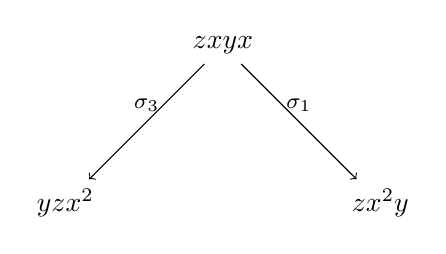
\begin{tikzpicture}
\node (1) at (0,0) {$zxyx$};
\node (a1) at (-2,-2) {$yzx^2$};
\node (a2) at (2,-2) {$zx^2y$};

\draw[->] (1) to node[above, font=\footnotesize]{$\sigma_3$} (a1);
\draw[->] (1) to node[above, font=\footnotesize]{$\sigma_1$} (a2);
\end{tikzpicture}
\]
and once again we are stuck, since both $yzx^2$ and $zx^2y$ are $S$-irreducible. One may try to enlarge the current set of rewriting rules as to include the new rule $zx^2y \rightsquigarrow yzx^2$, but this will in turn create another unresolvable ambiguity.

The problem is solved if we consider the rewriting system $S'$ composed of the rewriting rules:
\begin{align*}
\sigma &= yx \rightsquigarrow xy\\
\tau_n &= zx^ny \rightsquigarrow yzx^n
\end{align*}
for all $n\in\NN_0$. As we can see, the rewriting system $S'$ is compatible with the grlex monomial order, and since the identities $zx^ny=yzx^n$ hold in $A$, we have that $I_{S'} = (xy-yx, yzx^n-zx^ny)=(xy-yx, yz-zy)$. The rules $\tau_j$ and $\tau_k$ do not overlap or contain each other for any choice of $j$ and $k$, so the only overlapping ambiguities are of the form $(\tau_n,\sigma,zx^n,y,x)$, for $n\in\NN_0$. We now check that these ambiguities are resolvable:
\[
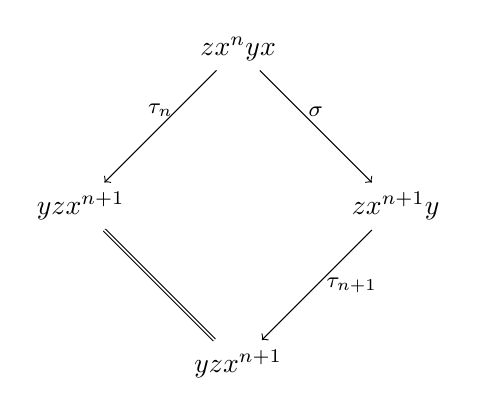
\begin{tikzpicture}
\node (1) at (0,0) {$zx^nyx$};
\node (a1) at (-2,-2) {$yzx^{n+1}$};
\node (a2) at (2,-2) {$zx^{n+1}y$};
\node (b) at (0,-4) {$yzx^{n+1}$};

\draw[->] (1) to node[above, font=\footnotesize]{$\tau_n$} (a1);
\draw[->] (1) to node[above, font=\footnotesize]{$\sigma$} (a2);
\draw[->] (a2) to node[right, font=\footnotesize]{$\tau_{n+1}$} (b);
\draw[double] (a1) to (b);
\end{tikzpicture}
\]\note{arreglar formato del dibujo}
Therefore, the rewriting system is confluent, and so the set of $S'$-irreducible monomials form a basis for the algebra $A$. In this case, characterizing this set is not as easy as in the previous examples, since the rewriting system is considerably more complex. This, of course, reflects the fact that the basis has a richer combinatorial structure.
\end{exmp}

We now summarize our usual method to produce confluent rewriting systems:

\begin{heur}\label{heuristic} Let $A=k\langle x_1,\dots,x_n\rangle/(r_1,\dots,r_m)$ be a $k$-algebra given by generators and relations. The lexicographic order $x_1<\dots<x_n$ induces a grlex monomial order $\preceq$ on $\langle x_1,\dots,x_n\rangle$, which satisfies the descending chain condition by \hyperref[noeth]{Lemma \ref*{noeth}}. We can produce a rewriting system following these steps:
\begin{enumerate}
\item Write each relation $r_i$ as
\[r_i = \lambda_{i,1}w_{i,1} + \lambda_{i,2} w_{i,2} + \dots + \lambda_{i,k_i} w_{i, k_i},\]
where $w_{i,j}\in \langle x_1,\dots,x_n\rangle$, $\lambda_{i,j}\in k$ and $w_{i,1}\succeq w_{i,2}\succeq\dots\succeq w_{i,k_i}$.
\item Consider the rules
\[\sigma_i = w_{i,1} \rightsquigarrow -\lambda_{i,1}^{-1}\lambda_{i,2}w_{i,2}-\dots-\lambda_{i,1}^{-1}\lambda_{i,k_i}w_{i,k_i}\]
which are all compatible with the monomial order $\preceq$ and are such that the rewriting system $S=\{\sigma_i\}$ induces the ideal $I_S=(r_1,\dots,r_m)$.
\item If all ambiguities arising from this rewriting system are resolvable, we are done. Otherwise, given an unresovable ambiguity $(\sigma_i, \sigma_j, u,v,w)$, reduce both $r_i(uv)w$ and $ur_j(vw)$ into irreducible elements, which we will call $a$ and $b$ respectively. We have that $a-b\in I_S$, and so \[A=k\langle x_1,\dots,x_n\rangle/(r_1,\dots,r_m)=k\langle x_1,\dots,x_n\rangle/(r_1,\dots,r_m, a-b).\]
Treating $a-b$ as another relation, we can follow the steps 1 and 2 as to produce a new rule that will solve the previous ambiguity, but may generate new ones.
\item Repeat step 3 until the system is confluent.
\end{enumerate}
This procedure, of course, does not always terminate in a finite number of steps, but is good enough as to solve most of the cases that arise throughout this thesis.
\end{heur}
\end{section}
\begin{section}{A diamond lemma for path algebras}
\label{path-diamond}
As seen in the previous section, Bergman's diamond lemma is a statement about certain quotients of free algebras. However, we will only apply it on a particular family of algebras, namely quotients of path algebras. Even though obviously path algebras are themselves quotients of free algebras, using Bergman's diamond lemma can be quite cumbersome in this case. For example, consider the following quiver, which we will name $Q$:
\[
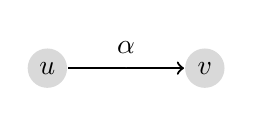
\begin{tikzpicture}[->,node distance=1cm, thick]
\tikzstyle{every node} = [circle, fill=gray!30, minimum size=.5cm, inner sep=.07cm]
\node (1) at (0,0) {$u$};
\node (2) at (2,0) {$v$};
\draw (1) -- (2) node[midway, above, fill=white] {$\alpha$};
\end{tikzpicture}
\]
The path algebra $\kQ$ may be described as the quotient of the free algebra $k\langle u,v,\alpha\rangle$ by the ideal
\[(\underbrace{uv, vu, u^2-u, v^2-v, u+v-1}_{\substack{\text{$u$ and $v$ are idempotent orthogonal}\\\text{elements of sum $1$}}}, \underbrace{\alpha^2, \alpha u-\alpha, v\alpha-\alpha, \alpha v,u\alpha }_{\substack{\text{relations forced by the way arrows}\\\text{and vertices concatenate}}})\]
Even in a quiver as simple as $Q$ and without introducing further relations in the path algebra, a lot of rewriting rules and ambiguities arise. Therefore, it makes sense to produce a specialized version of the diamond lemma in order to deal with this particular case in a more efficient manner, in a similar vein as \cite{FFG93}.

Given a quiver $Q$, a \emph{rewriting system} on $Q$ is a subset $S\subseteq Q_*\times \kQ$, where $Q_*$ stands for the set of all paths on $Q$. A \emph{path order} on $Q_*$ is a partial order $\preceq$ on $Q_*$ such that if $v$ and $v'$ are parallel paths (that is, they share the same source and target) and $v\preceq v'$, then $uvw\preceq uv'w$ for all $u,w\in Q_*$ with appropriate source and target. All other previous definitions translate almost verbatim to this new setting. We now are able to formulate our specialized version of the diamond lemma:

\begin{thm}\label{quiver-diamond-lemma} Let $Q$ be a quiver, $S$ be a rewriting system for $Q$ and $\preceq$ a path order on $Q_*$ compatible with $S$ and satisfying the descending chain condition. Let $I_S$ be the ideal given by the relations induced by $S$, that is, $I_S=(w_\sigma-f_\sigma)_{\sigma\in S}$. Then the following conditions are equivalent:
\begin{enumerate}
\item All ambiguities of $S$ are resolvable.
\item All elements of $\kQ$ are reduction-unique under $S$.
\item A set of representatives in $\kQ$ for the elements of the algebra $\kQ/I_S$ is given by the $k$-submodule $\kQ_{\mathrm{irr}}$ spanned by the $S$-irreducible paths of $Q_*$.
\end{enumerate}
If any of these conditions hold, the rewriting system $S$ is said to be $\emph{confluent}$. In that case, there is a $k$-algebra isomorphism between $\kQ/I_S$ and $\kQ_{\mathrm{irr}}$, where the latter is a $k$-algebra with product defined as $x\cdot y= r_S(xy)$.
\end{thm}\note{chequear el enunciado}

\begin{exmp} Consider the quiver $Q$ given by the following diagram:
\[
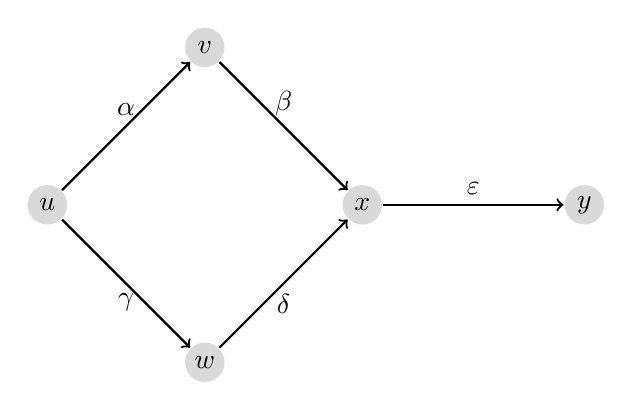
\begin{tikzpicture}[->,node distance=1cm, thick]
\tikzstyle{every node} = [circle, fill=gray!30, minimum size=.5cm, inner sep=.07cm]
\node (1) at (0,0) {$u$};
\node (2) at (2,2) {$v$};
\node (3) at (2,-2) {$w$};
\node (4) at (4,0) {$x$};
\node (5) at (6.82,0) {$y$};
\tikzstyle{every node} = []
\draw (1) -- (2) node[midway, above] {$\alpha$};
\draw (2) -- (4) node[midway, above] {$\beta$};
\draw (1) -- (3) node[midway, below] {$\gamma$};
\draw (3) -- (4) node[midway, below] {$\delta$};
\draw (4) -- (5) node[midway, above] {$\varepsilon$};
\end{tikzpicture}
\]
We will make use of the diamond lemma to produce a basis for the algebra $A=\kQ/(\delta\gamma-\beta\alpha, \varepsilon\beta, \varepsilon\delta)$. The usual grlex ordering induced by the lexicographical order suggests the rewriting rules:
\begin{align*}
\sigma_1 &= \delta\gamma \rightsquigarrow \beta\alpha\\
\sigma_2 &= \varepsilon\beta \rightsquigarrow 0\\
\sigma_3 &= \varepsilon\delta \rightsquigarrow 0
\end{align*}
Thus, the rewriting system $S=\{\sigma_1,\sigma_2,\sigma_3\}$ presents a unique ambiguity, which is $(\sigma_3,\sigma_1, \varepsilon,\delta,\gamma)$. The following diagram shows that this ambiguity is resolvable:
\[
\begin{tikzpicture}
\node (1) at (0,0) {$\varepsilon\delta\gamma$};
\node (a1) at (-2,-2) {$0$};
\node (a2) at (2,-2) {$\varepsilon\beta\alpha$};
\node (b) at (0,-4) {$0$};

\draw[->] (1) to node[above, font=\footnotesize]{$\sigma_3$} (a1);
\draw[->] (1) to node[above, font=\footnotesize]{$\sigma_1$} (a2);
\draw[->] (a2) to node[below, font=\footnotesize]{$\sigma_2$} (b);
\draw[double] (a1) to (b);
\end{tikzpicture}
\]
The rewriting system $S$ is confluent, and our algebra $A$ has a basis given by the $S$-irreducible paths, which are
\[\{e_u, e_v, e_w, e_x, e_y, \alpha,\beta,\gamma,\delta,\varepsilon, \beta\alpha \},\]
where $e_a$ stands for the stationary path at the vertex $a$.
\end{exmp}
\begin{exmp} Let $Q$ be the following quiver:
\[
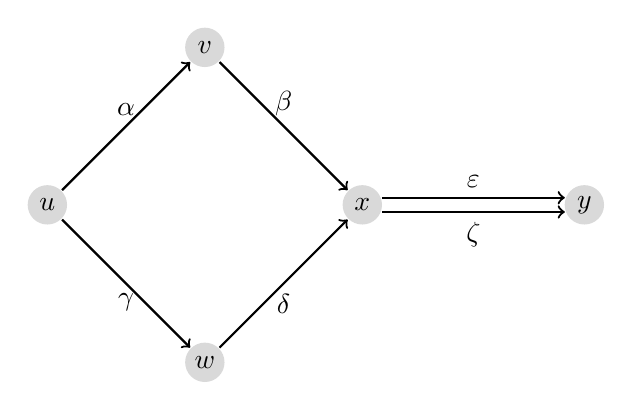
\begin{tikzpicture}[->,node distance=1cm, thick]
\tikzstyle{every node} = [circle, fill=gray!30, minimum size=.5cm, inner sep=.07cm]
\node (1) at (0,0) {$u$};
\node (2) at (2,2) {$v$};
\node (3) at (2,-2) {$w$};
\node (4) at (4,0) {$x$};
\node (5) at (6.82,0) {$y$};
\tikzstyle{every node} = []
\draw (1) -- (2) node[midway, above] {$\alpha$};
\draw (2) -- (4) node[midway, above] {$\beta$};
\draw (1) -- (3) node[midway, below] {$\gamma$};
\draw (3) -- (4) node[midway, below] {$\delta$};
\draw (4.20) -- (5.160) node[midway, above] {$\varepsilon$};
\draw (4.340) -- (5.200) node[midway, below] {$\zeta$};
\end{tikzpicture}
\]
Consider the algebra $A=\kQ/(\delta\gamma-\beta\alpha, \varepsilon\beta, \zeta\delta)$. Following our usual procedure, we first consider the rewriting system $S$ given by the rules
\begin{align*}
\sigma_1 &= \delta\gamma \rightsquigarrow \beta\alpha\\
\sigma_2 &= \varepsilon\beta \rightsquigarrow 0\\
\sigma_3 &= \zeta\delta \rightsquigarrow 0
\end{align*}

In this case, the rewriting system is not confluent, since the ambiguity $(\sigma_3, \sigma_1, \zeta, \delta, \gamma)$ is unresolvable. However, after enlarging the system as to contain the rule
\[\sigma_4 = \zeta\beta\alpha\rightsquigarrow 0,\]
we achieve confluence. Thus, a basis is given by the $S$-irreducible monomials.
\end{exmp}
\end{section}

\begin{section}{A topological diamond lemma}
As Jacobian algebras are quotients of completed path algebras by closed ideals, one needs to further specialize the diamond lemma in order to account for issues of convergence, as carried out in the works \cite{Hel02} and \cite{SAV15}.

Most of the terminology needed to introduce this last version of the lemma has already been presented; we will only need to provide a slight variation on the descending chain condition. We say that a monomial order $\preceq$ satisfies the \emph{descending chain condition in norm} if every sequence $(x_n)$ of monomials in $\mon$ such that $x_{n+1}\prec x_n$ for all $n\geq 0$ converges to zero in $k\llangle X\rrangle$.

\begin{thm} Let $X$ be a set, $S$ be a rewriting system for $X$ and $\preceq$ a monoid order on $\mon$ compatible with $S$ and satisfying the descending chain condition in norm. Let $I_S$ be the closed ideal given by the relations induced by $S$, that is, $I_S=\overline{(w_\sigma-f_\sigma)}_{\sigma\in S}$. Then the following conditions are equivalent:
\begin{enumerate}
\item All ambiguities of $S$ are resolvable.
\item All elements of $k\llangle X\rrangle$ are reduction-unique under $S$.
\item A set of representatives in $k\llangle X\rrangle$ for the elements of the algebra $k\llangle X\rrangle/I_S$ is given by the closed $k$-submodule $k\llangle X\rrangle_{\mathrm{irr}}$ spanned by the $S$-irreducible monomials of $\mon$.
\end{enumerate}
Once again, if any of these conditions hold, the rewriting system $S$ is said to be $\emph{confluent}$, and in that case  there is a $k$-algebra isomorphism between $k\llangle X\rrangle/I_S$ and $k\llangle X\rrangle_{\mathrm{irr}}$, where the latter is a $k$-algebra with product defined as $x\cdot y= r_S(xy)$.
\end{thm}

A similar statement for quotients of complete path algebras may be produced as well. Indeed, one may modify the statement of \hyperref[quiver-diamond-lemma]{Theorem \ref*{quiver-diamond-lemma}} replacing "descending chain condition" by "descending chain condition in norm" and all algebraic objects by their complete counterparts (algebras and their completions, ideals and closed ideals, submodules and closed submodules, etc.) to obtain the result.

Given a total order $\leq$ on a set $X$, the \emph{reverse graded lexicographical order}, or \emph{revglex} for short, is the monomial order $\preceq$ defined on $\mon$ as follows: given $u,v\in \mon$, we have $u\preceq v$ if
\begin{itemize}
\item $|u| > |v|$ or
\item $|u| = |v|$ and $u=wau'$, $v=wbv'$, with $w,u',v'\in \mon$, $a,b\in X$ and $a\leq b$.
\end{itemize}
Therefore, monomials are sorted first by length (but this time longer terms are smaller with respect to $\preceq$) and then lexicographically according to the total order $\leq$. Analogously one defines the revglex order for paths on a quiver. This will be our preferred order when dealing with completions, since we have that:

\begin{lemma}\label{noeth-norm}Let $(X,\leq)$ be a finite, totally ordered set. Then, the revglex order on $\mon$ satisfies the descending chain condition in norm.
\end{lemma}
\begin{proof} Let $(x_n)$ be a strictly decreasing sequence in $\mon$ and $k$ be the cardinality of $X$. There are exactly $j=\sum_{l=0}^d k^l$ words in $\mon$ of length at most $d$, and so $x_{j+1}$ must be of length at least $d+1$, since the sequence $(x_n)$ is strictly decreasing. Thus, in $k\llangle X\rrangle$ we have that $\Vert x_{n}\Vert\leq e^{-d-1}$ for all $n\geq j+1$ and so $x_n\rightarrow 0$ as we wanted.
\end{proof}

Once again, an analogous result holds for quivers and complete path algebras.

\begin{exmp} In general, given an ideal $I$, the algebras $k\langle X\rangle/I$ and its completed counterpart $k\llangle X\rrangle/\overline{I}$ may be quite different. For instance, consider the ideal $I=(x^2-x)$ in $k\langle x \rangle$. We may form the algebras $A=k\langle x\rangle/I$ and $B=k\llangle x\rrangle/\overline{I}$.

Since we know that $(x^2-x)=(x)\cap(x-1)$ and the ideals $(x)$ and $(x-1)$ are coprime, by the chinese remainder theorem we have that
\[A=\frac{k\langle x\rangle}{(x^2-x)}\simeq \frac{k\langle x\rangle}{(x)} \times \frac{k\langle x\rangle}{(x-1)}\simeq k\times k.\]
We now study $B$ using the diamond lemma. The rewriting system $S=\{x\rightsquigarrow x^2\}$ is compatible with the reverse graded path order and is obviously confluent, since the monomial $x$ does not overlap with itself in any non-trivial way. We see that the only $S$-irreducible monomials are the constant ones, and so a basis for $B$ is given by $\{[1]\}$, and thus $B\simeq k$.

More generally, if $I=(x^n-x)$, we have that
\[\frac{k\langle x\rangle}{(x^n-x)} \simeq \frac{k\langle x\rangle}{(x)}\times \frac{k\langle x\rangle}{(x^{n-1}-1)}\simeq k \times \frac{k\langle x\rangle}{(x^{n-1})},\]
which is an $n$-dimensional algebra, while in the completed case we have that $k\llangle x\rrangle/\overline{I}\simeq k$ by the same reasoning as above, since the rewriting system $S=\{x\rightsquigarrow x^n\}$ is confluent.
\end{exmp}
\end{section}
\end{chapter}